\documentclass[border=2pt]{standalone}
% Shared preamble of the standalone figures of Paper2_V28 (journal artwork rules: Helvetica
% lettering, 8-9 pt at final size, lines >= 0.4 pt, colorblind-safe RGB colors plus patterns).
\usepackage[T1]{fontenc}
\usepackage[scaled=0.95]{helvet}
\renewcommand{\familydefault}{\sfdefault}
\usepackage[helvet]{sfmath}
\usepackage{textcomp}
\usepackage{tikz}
\usepackage{pgfplots}
\pgfplotsset{compat=1.17}
\usetikzlibrary{arrows.meta,calc,positioning,patterns}
\definecolor{okblue}{HTML}{0072B2}
\definecolor{okverm}{HTML}{D55E00}
\definecolor{okgray}{HTML}{9A9A9A}
\definecolor{oklight}{HTML}{D9D9D9}
\definecolor{okdark}{HTML}{4D4D4D}

\begin{document}
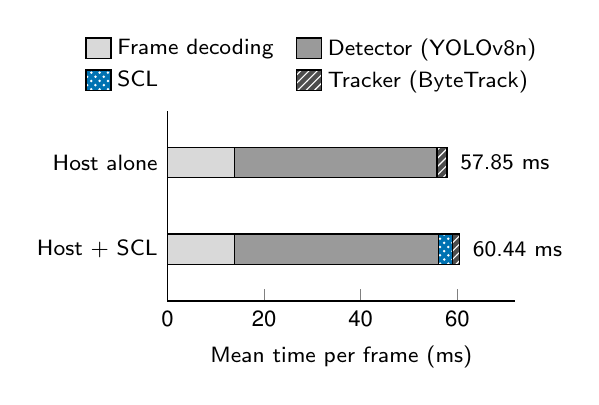
\begin{tikzpicture}
\begin{axis}[
  xbar stacked, /pgf/bar width=11pt, width=6.0cm, height=4.0cm,
  xmin=0, xmax=72, clip=false, ymin=-0.6, ymax=1.6,
  ytick={0,1}, yticklabels={Host + SCL, Host alone},
  xlabel={Mean time per frame (ms)},
  axis x line*=bottom, axis y line*=left, axis line style={line width=0.6pt},
  tick label style={font=\footnotesize}, label style={font=\footnotesize},
  legend style={at={(0.42,1.04)}, anchor=south, legend columns=2, font=\footnotesize, draw=none,
    /tikz/every even column/.append style={column sep=6pt}},
  legend image code/.code={\draw[#1] (0cm,-0.12cm) rectangle (0.32cm,0.14cm);},
  legend cell align=left,
]
\addplot[fill=oklight, draw=black, line width=0.5pt] coordinates {(13.88,1) (13.88,0)};
\addplot[fill=okgray, draw=black, line width=0.5pt] coordinates {(41.91,1) (42.17,0)};
\addplot[fill=okblue, draw=black, line width=0.5pt, postaction={pattern=crosshatch dots, pattern color=white}] coordinates {(0,1) (2.95,0)};
\addplot[fill=okdark, draw=black, line width=0.5pt, postaction={pattern=north east lines, pattern color=white}] coordinates {(2.04,1) (1.43,0)};
\legend{Frame decoding, Detector (YOLOv8n), SCL, Tracker (ByteTrack)}
\node[anchor=west, font=\footnotesize] at (axis cs:58.6,1) {57.85 ms};
\node[anchor=west, font=\footnotesize] at (axis cs:61.2,0) {60.44 ms};
\end{axis}
\end{tikzpicture}
\end{document}
